\documentclass[onecolumn, draftclsnofoot,10pt, compsoc]{IEEEtran}
\usepackage{graphicx}
\usepackage{url}
\usepackage{setspace}
\usepackage{float}
\usepackage{array,multirow}
\usepackage{tabularx,graphicx}

\usepackage{geometry}
\geometry{textheight=9.5in, textwidth=7in}

% 1. Fill in these details 
\def \CapstoneTeamName{		Know It's Off Software Team}
\def \CapstoneTeamNumber{		34}
\def \GroupMemberOne{			Tristan Jong}
\def \GroupMemberTwo{			Ben Martin}
\def \GroupMemberThree{			Kyle Peterson}
\def \CapstoneProjectName{	    Know It's Off}
\def \CapstoneSponsorCompany{	Oregon State University}
\def \CapstoneSponsorPerson{		Donald Heer}

% 2. Uncomment the appropriate line below so that the document type works
\def \DocType{		%Problem Statement
				%Requirements Document
				%Technology Review
				%Design Document
				Final Progress Report
				}
			
\newcommand{\NameSigPair}[1]{\par
\makebox[2.75in][r]{#1} \hfil 	\makebox[3.25in]{\makebox[2.25in]{\hrulefill} \hfill		\makebox[.75in]{\hrulefill}}
\par\vspace{-12pt} \textit{\tiny\noindent
\makebox[2.75in]{} \hfil		\makebox[3.25in]{\makebox[2.25in][r]{Signature} \hfill	\makebox[.75in][r]{Date}}}}
% 3. If the document is not to be signed, uncomment the RENEWcommand below
\renewcommand{\NameSigPair}[1]{#1}

%%%%%%%%%%%%%%%%%%%%%%%%%%%%%%%%%%%%%%%
\begin{document}
\begin{titlepage}
    \pagenumbering{gobble}
    \begin{singlespace}
        \hfill 
        % 4. If you have a logo, use this includegraphics command to put it on the coversheet.
        %\includegraphics[height=4cm]{CompanyLogo}   
        \par\vspace{.2in}
        \centering
        \scshape{
            \huge CS Capstone \DocType \par
            {\large\today}\par
            \vspace{.5in}
            \textbf{\Huge\CapstoneProjectName}\par
            \vfill
            {\large Prepared for}\par
            \Huge \CapstoneSponsorCompany\par
            \vspace{5pt}
            {\Large\NameSigPair{\CapstoneSponsorPerson}\par}
            {\large Prepared by }\par
            Group\CapstoneTeamNumber\par
            % 5. comment out the line below this one if you do not wish to name your team
            \CapstoneTeamName\par 
            \vspace{5pt}
            {\Large
                \NameSigPair{\GroupMemberOne}\par
                \NameSigPair{\GroupMemberTwo}\par
                \NameSigPair{\GroupMemberThree}\par
            }
            \vspace{20pt}
        }
        
    \end{singlespace}
\end{titlepage}
\newpage
\pagenumbering{arabic}
\tableofcontents
% 7. uncomment this (if applicable). Consider adding a page break.
%\listoffigures
%\listoftables
\clearpage

\section{Project Purposes and Goals}


% 8. now you write!https://www.overleaf.com/project/5de80908f9c547000177d214
\quad The Know It's Off Project aims to produce a system that helps users keep track of the on and off status of electronic appliances in their house. Current options for consumers to track this include expensive "smart home" appliances such as a Samsung Smart Stove that have many other functionalities on top of tracking on/off status. This project's purpose is to provide just the ability to track if the appliance is on or off, but through much more affordable means. 

Users attach small devices known as scouts to appliances such as electric stoves, coffee makers, or laundry machines. After doing so, users can check a web application which keeps a history of the on/off status of these machines for the user to view. They can also check the battery life of each scout to know when to replace the batteries, or reassign the scouts to different appliances if they are moved. The system also has the ability to send text message notifications to users about their appliance status. Security measures are implemented as well to prevent outside sources from exploiting the system to harm consumers. 

The Know It's Off Project consists of a computer science team which works mainly on the web application, server, and database, as well as an ECE team which works on the functionalities of the scout. 

\section{Current Progress}

\subsection{Web Application}
We have developed a working UI and backend with almost all planned functionalities completed. Users can access the web application from a browser, with the web server hosted on Oregon State University's ENGR servers. Upon going to the web application, the landing page is a login where users can either log in or create an account if they do not have one yet. Once a user has logged in, they can view a history of their appliance status.  

\subsection{Text and Email Notifications}
When devices are left on for a specified amount of time, an automated messaging system will trigger and message the user's email and phone, depending on whether they activated email and text message alerts. We have included a small snippet of code of the function checking the message queue on the database and sending alerts as necessary. We used Twilio for text messaging, and a google email account to send automated emails.

\begin{figure}
    \centering
    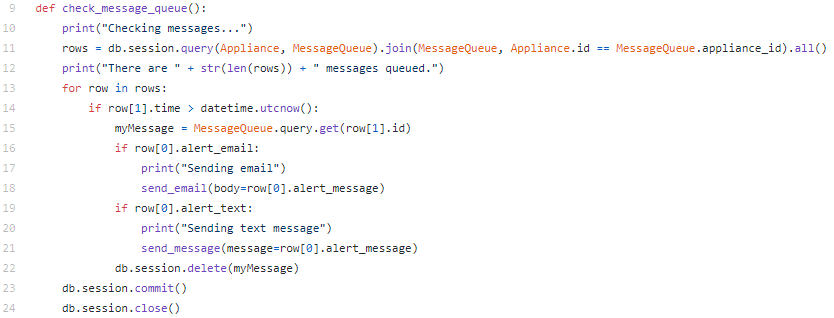
\includegraphics[width = \textwidth]{message.PNG}
    \caption{Behind the scenes code of the background thread checking the message queue and sending messages if the time has expired for each appliance.}
\end{figure}

\begin{figure}
    \centering
    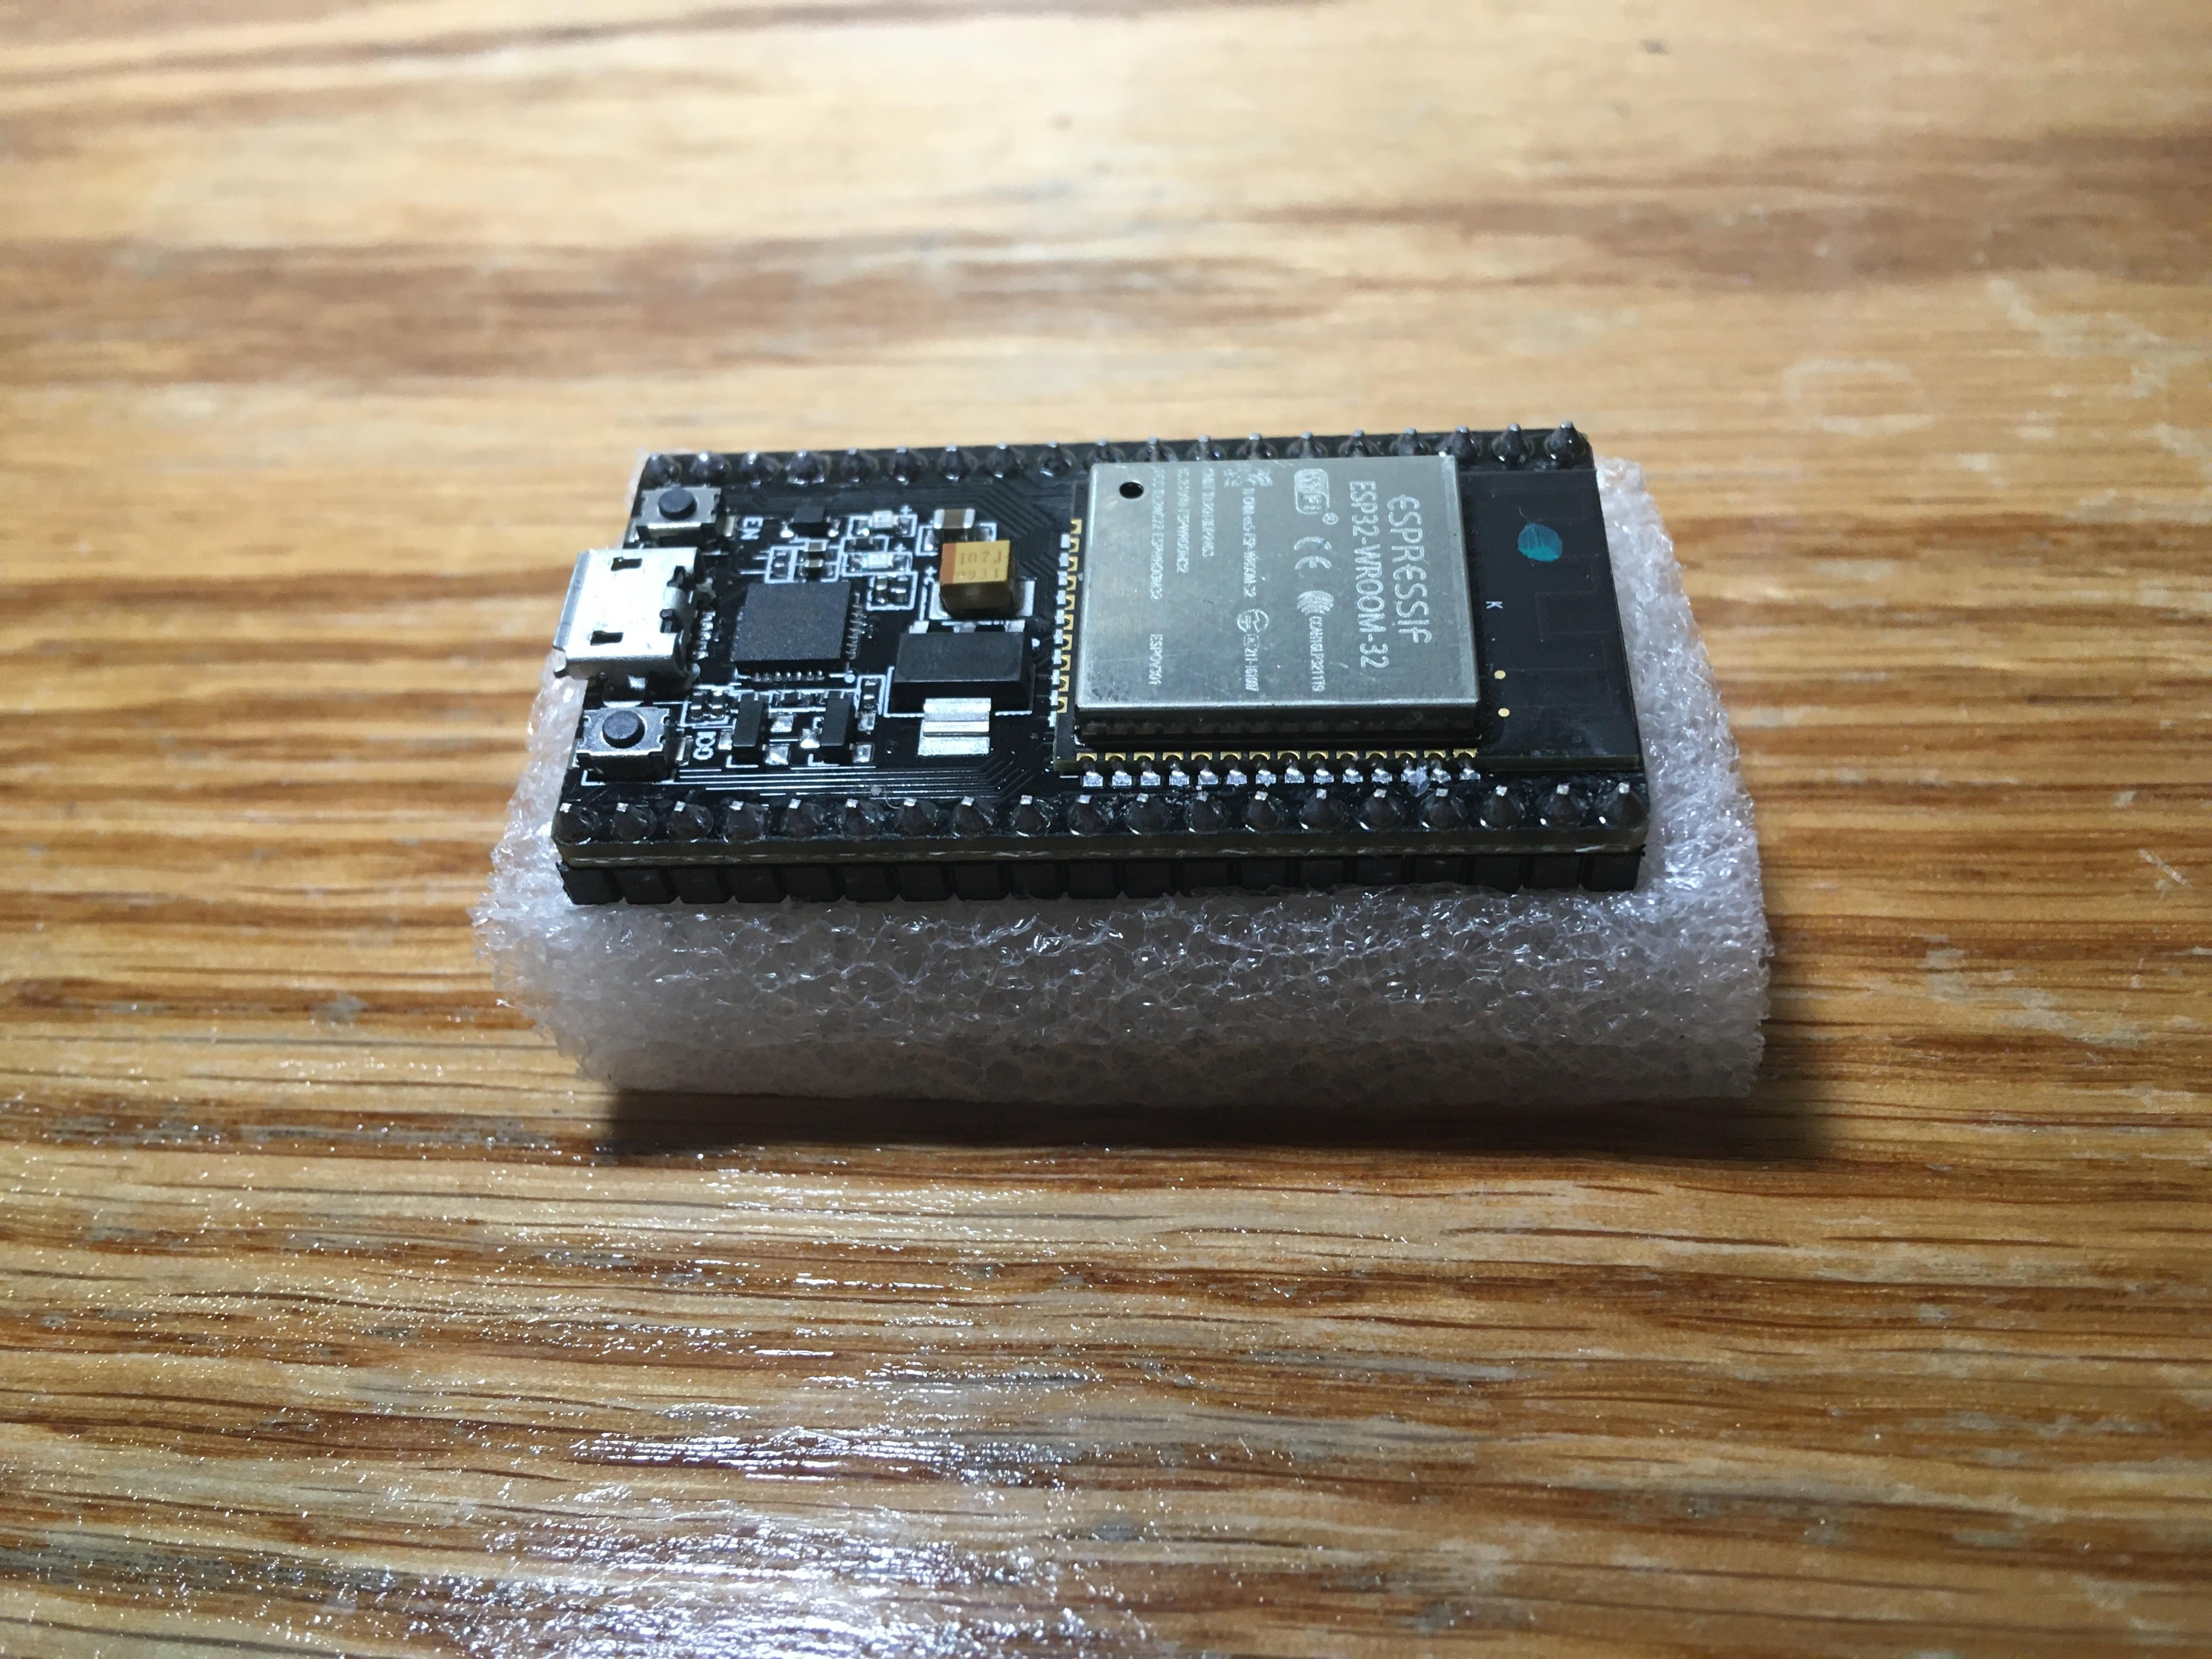
\includegraphics[width = \textwidth]{unnamed.jpg}
    \caption{Image of ESP32 device, similar to the ESP8266, which the ECE team is using.}
\end{figure}

\subsection{Scout Communication}
Scouts communicate one-way to the server. This means that the server does not send messages back to the scout, and the scout cannot receive messages and instead only sends POST or PATCH requests to the server. Currently, our test scout cannot sense changes in the appliance it is attached to, but it can send requests to the server that we can correctly receive. The ECE team is responsible for the appliance-sensing functionalities of the scout as well as its ability to send requests to the server based on what it senses. 

\subsection{Security Features}
Since the web application is hosted on the ENGR servers, the landing page can be configured to force HTTPS connections which is planned but has not yet happened. This feature can be implemented very quickly though. When a user creates an account, their password is hashed using the SHA-256 hashing algorithm before being stored in the user table of the database. Hashing is a process where an input string is processed into an output string that is not meant to be reversible. That is, that it is very difficult to figure out what the output string's original input string was. By hashing the password before storing it, attackers who could get access to the user table of the database would still not be able to easily figure out a matching password to a corresponding username. 

When a user registers a scout to their account on the web application, the scout's id is paired with the user's account. The user will not accept potential fake transmissions that do not originate from scouts paired with that specific user. After the user has logged in and paired the scout with their account, the scout will be given the authentication token for the server. This will allow the server to identify which scout is sending any messages it receives and also to verify that the sender is not an outside attacker pretending to be a scout because only the scout would hold the authentication token. 

\subsection{Google Home Interfacing}

We currently have a DialogFlow Agent which can properly interact and respond to queries, but it needs to be integrated with the API on the backend. There are two intents that can be expressed by the user: "Is my appliance X on?", and "Is my appliance Y off?". If the user has more than one appliance, then the name or type of appliance must be specified. If there is more than one appliance of the same type, then the name of the appliance must be identified. (The user must uniquely name each appliance that they register under the Know It's Off system).

\begin{figure}
    \centering
    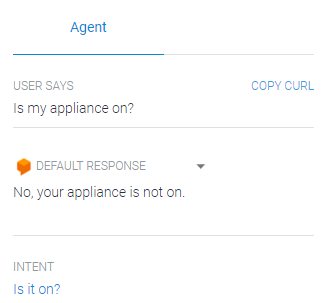
\includegraphics{applianceOff.PNG}
    \caption{Results of querying appliance state}
\end{figure}

\begin{figure}
    \centering
    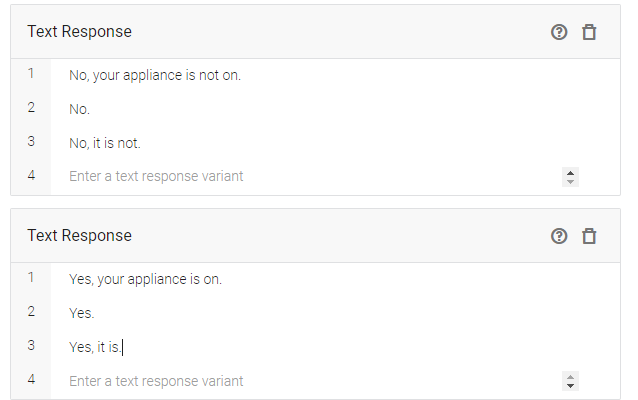
\includegraphics{applianceResponse.PNG}
    \caption{Response variations for a user's intent on the "Is it on?" intent.}
\end{figure}


\section{Roadblocks and Issues}

\subsection{Database Connections Issue}
A recurring problem we faced was that when the database tried to make a connection, it was sometimes refused because the server only up to four connections per the settings laid out by OSU for their ENGR servers. This should be more than enough, and in our code we made sure to close out every database connection we made as soon as we were done with it. For some reason though, through multiple hours of troubleshooting, we were still unable to fix it. We do not know where the extra connections are coming from or if our previous connections are being closed. Our only current solution is to restart to clear all the connections and then retry, and we do not currently have a known solution we can work towards that would be a permanent fix. OSU IT does not know either. 

\subsection{Flask-Login Implementation}
Flask-login is a package for our backend that helps manage user login sessions. We had previously tried to implement it this term but had to do a code rollback because it was buggy before our group presentation where we needed to demo alpha functionality. Along with rolling this back we also lost the password hashing implementation. We plan to refactor our user session-related code and to implement flask-login again because a correct implementation will handle user sessions much better and more conveniently than how we currently have it set up. after we have implemented flask-login correctly, we should be able to quickly and easily introduce the password hashing as 

\end{document}